% polyhedron.tex
% ------------------------------------------------------------------------
\label{sec:poly}

% The design of \cgalpoly\ consists of four components:

\paragraph*{A Geometric Traits Concept} is defined for \cgalpoly\ that
describes the types for geometric primitives, predicates and
constructions. Relevant for us is the point type defined here. A
\cgal\ kernel is a valid model.

\paragraph*{Items}  are collectively the  vertices, halfedges, and
facets. They contain the pointers referring to incident items (see
Fig.~\ref{fig:halfedge}) and the additional attributes including the
geometry, such as points in vertices. Mandatory for \cgalpoly\ are the
\CodeFmt{next}, \CodeFmt{opposite}, and \CodeFmt{vertex} incidence
pointers, and a three-dimensional point in vertices. All other
incidences, also the back pointers from a vertex or facet to an
incident halfedge, are optional, but if they are provided, they will
be automatically maintained in all operations. By default all
incidences are provided plus a plane equation in facets.

In fact, the design does not use pointers, but %the abstraction of
\emph{handles}, a.k.a. the \emph{trivial iterator\/} concept that
requires the dereference operator, but no traversal of a sequence.
These handle types are also available to the user when they extend items
with additional attributes and references.
%, e.g., material properties
%for rendering or links in multi-resolution representations.

\paragraph*{The Halfedge Data Structure} is a container class managing
the storage for items. Two solutions are provided; one stores items in
a list that allows for efficient insertion and removal, and one
stores items in an array that allows random access and more compact
storage, but is less flexible in removing and inserting items, e.g.,
inserting items beyond the currently reserved capacity causes the
array to reallocate and update all invalidated handles.

The type dependency between the different item types is not hardcoded
on the items level. Instead, the halfedge data structure defines the
iterator and handle types and instantiates the items with these types.
This gives great flexibility in extending and exchanging individual
item types. The internal realization of this design is a brain
twister, but the user is not exposed to it and we skip details and refer
to~\cite{k-ugpdd-99}.

\begin{figure}[tb]
  \centering
  \psfrag{PQQ}[]{\scriptsize PQQ} 
  \psfrag{PTQ}[]{\scriptsize PTQ}
  \psfrag{DQQ}[]{\scriptsize DQQ} 
  \psfrag{Sqrt3}[]{\scriptsize $\sqrt{3}$} 
  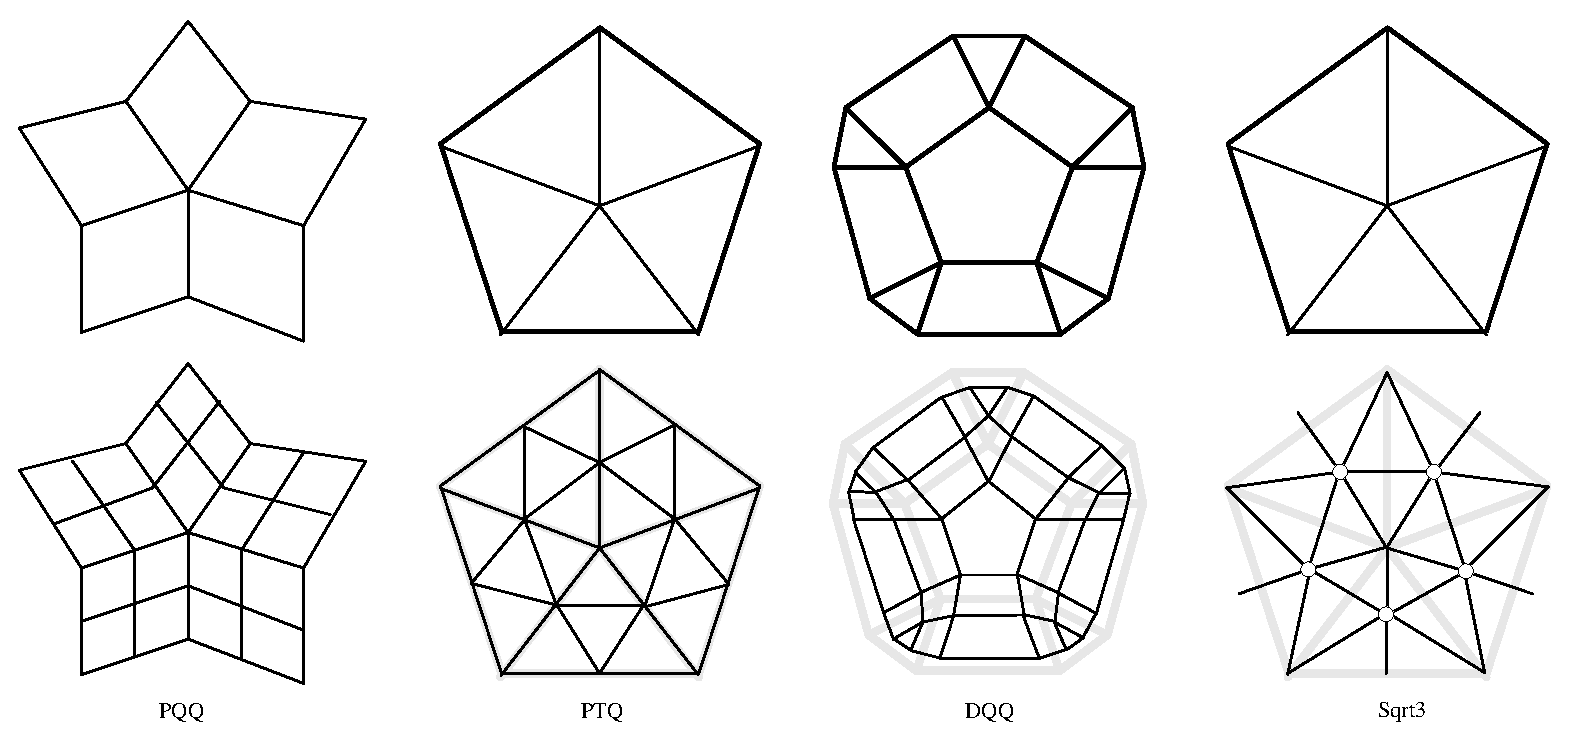
\epsfig{file=figs/RefSchemes.eps, width=7cm}
  \caption{Examples of refinement schemes: 
    primal quadrilateral quadrisection (PQQ),
    primal triangle quadrisection (PTQ),
    dual quadrilateral quadrisection (DQQ) and
    $\sqrt{3}$ triangulation. The control meshes are shown
    in the first row.}
  \label{fig:RefSchemes}\vspace*{-4mm}
\end{figure}



\paragraph*{CGAL::Polyhedron\_3} is the top-level interface class that
assembles the other pieces in a convenient user-friendly interface.
It offers iterators for all items and defines \emph{circulators} for
the circular sequence of halfedges around a vertex and for halfedges
around a facet. Circulator is a new concept in \cgal\ that
corresponds closely to iterators, but is tailored for circular
sequences.  The main difference to iterators is the lack of a
past-the-end position that leads to the typical idiom of a
do-while-loop instead of the usual while-loop for iterators.  Let us
write a small function rendering a polyhedral surface with convex
facets in OpenGL with double coordinates in non-reference counted
points and making a bold, but informed guess about its memory layout.
Note that circulators and iterators have implicit conversions to the
corresponding handle types.
%\pagebreak
%\vspace*{-6mm}

\begin{lstlisting}
typedef Polyhedron_3<Simple_cartesian<double> > Polyhedron;
void render( const Polyhedron& P) {
  Polyhedron::Facet_const_iterator i;
  for ( i = P.facets_begin(); i != P.facets_end(); ++i) {
    glBegin( GL_POLYGON);
    Polyhedron::Halfedge_around_facet_const_circulator c = 
        i->facet_begin();
    do {
      glVertex3dv( & (c->vertex()->point().x()));
    } while ( ++c != i->facet_begin());
    glEnd();
  }
}
\end{lstlisting}%
\vspace*{-3.5mm}

\noindent
The sequential access is conventional, but the connectivity
modifications needs new ideas. The polyhedron protects the
combinatorial integrity of the underlying halfedge data structure.
Instead of updating individual handles in the items, it offers an
interface with Euler operations, so called because they preserve the
Euler-Poincar\'e invariance of a mesh. Examples of Euler operations
are the well-known edge collapse, split facet, and more.
\cite{Maentylae88} shows that all meshes can be created from a
suitable set of Euler operations.

Nevertheless, Euler operations can be cumbersome for certain tasks,
especially if a mesh operation needs to work with intermediate invalid
states of the halfedge data structure. The \cgalpoly\ provides a
backdoor access with the \CodeFmt{CGAL::Modifier} class to the
underlying halfedge data structure, but assures that, when this access
finishes, the integrity of the data structure is checked.

The prime example for this backdoor use is an alternative way of
describing meshes in the indexed-facet-set format that is common in file
formats: First, points are defined with their coordinates, then facets
are defined as sequence of indices to the points on their boundary. An
efficient implementation of such a construction is provided with the
incremental builder class in \cgal. 
%Examples for the different ways of
%modifying the mesh are given in the following sections.









